\newcommand{\timetosinglesolution}{
%Time for finding a single solution for a N-Sequencer
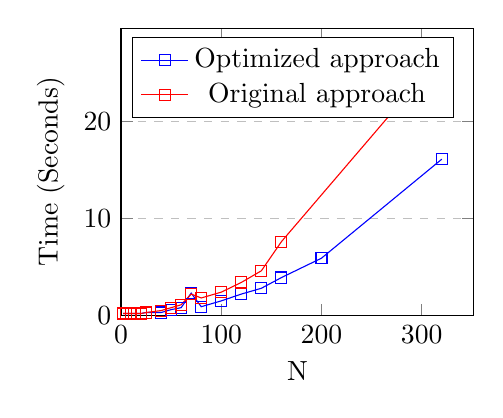
\begin{tikzpicture}
    \begin{axis}[width=0.5\textwidth,legend pos=north west,
            xlabel={N},
            ylabel={Time (Seconds)},
            xmin=0, %xmax=160,
            ymin=0, %ymax=580,
            %xtick={0,2,5,10,20,40,50,60,80,100,120,160},
            %ytick={0,20,40,60,80,100,120},
            ymajorgrids=true,
            grid style=dashed,
            %legend style={font=\fontsize{40}{50}\selectfont}, 
        ]
        \addplot[
            color=blue,
            mark=square,
        ]
        coordinates {
        (2,0.2)(5,0.2)(10,0.2)(20,0.2)(25,0.3)(40,0.3)(50,0.6)(60,0.8)(70,2.3)(80,.9)(100,1.5)(120,2.2)(140,2.8)(160,3.9)(200,5.9)(320,16.1)
        };
        \addlegendentry{Optimized approach}
        \addplot[
            color=red,
            mark=square,
        ]
        coordinates {
        (2,0.2)(5,0.2)(10,0.2)(20,0.2)(25,0.3)(40,0.5)(50,0.8)(60,1.1)(70,2.2)(80,1.8)(100,2.4)(120,3.4)(140,4.6)(160,7.6)(320,26.9)
        };
        \addlegendentry{Original approach}
    \end{axis}
\end{tikzpicture}
}

\newcommand{\constraintssize}{
%Size of the RCSP constraints for a N-Sequencer
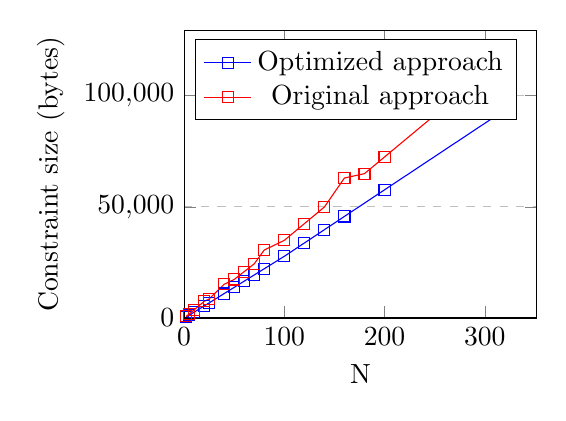
\begin{tikzpicture}
    \begin{axis}[width=0.5\textwidth,legend pos=north west,
        xlabel={N},
        ylabel={Constraint size (bytes)},
        xmin=0,% xmax=460,
        ymin=0, %ymax=200000,
         %xtick={0,2,5,10,20,40,50,60,80,100,120,160},
   %     ytick={0,20,100,1000,5000,50000,100000},
      %  legend pos=north west,
       ymajorgrids=true,
       grid style=dashed,
      %  legend style={font=\fontsize{10}{12}\selectfont}
%,
yticklabel style={
/pgf/number format/fixed}, scaled ticks=false
]
    \addplot[
        color=blue,
        mark=square,
    ]
    coordinates {
        (2,511)(5,1288)(10,2603)(20,5393)(25,6788)(40,10973)(50,13763)(60,16553)(70,19343)(80,22133)(100,27729)(120,33709)(140,39689)(160,45669)(200,57629)(320,93509)
    };
    \addlegendentry{Optimized approach}
    \addplot[
        color=red,
        mark=square,
    ]
    coordinates {
        (2,711)(5, 1788)(10,3609)(20,7459)(25,8552)(40,15159)(50,17327)(60,20837)(70,24347)(80,30559)(100,34901)(120,42401)(140,49901)(160,62945)(180,64901)(200,72401)(320,117401)
        };
        \addlegendentry{Original approach}
    \end{axis}
\end{tikzpicture}}


\newcommand{\ooooconstraintssize}{
%Size of the RCSP constraints for a N-Sequencer
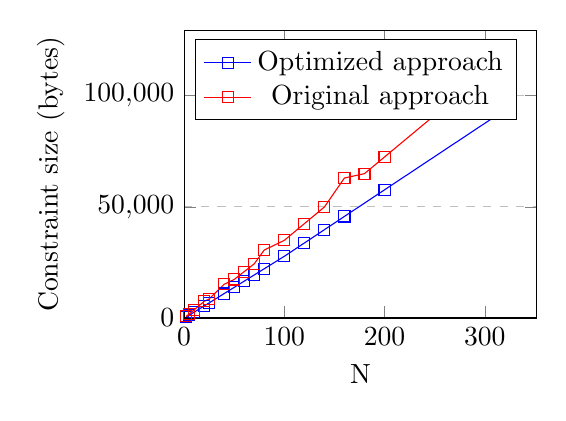
\begin{tikzpicture}
    \begin{axis}[width=0.5\textwidth,legend pos=north west,
        xlabel={N},
        ylabel={Constraint size (bytes)},
        xmin=0,% xmax=460,
        ymin=0, %ymax=200000,
         %xtick={0,2,5,10,20,40,50,60,80,100,120,160},
   %     ytick={0,20,100,1000,5000,50000,100000},
      %  legend pos=north west,
       ymajorgrids=true,
       grid style=dashed,
      %  legend style={font=\fontsize{10}{12}\selectfont}
%,
yticklabel style={
/pgf/number format/fixed}, scaled ticks=false
]
    \addplot[
        color=blue,
        mark=square,
    ]
    coordinates {
        (2,511)(5,1288)(10,2603)(20,5393)(25,6788)(40,10973)(50,13763)(60,16553)(70,19343)(80,22133)(100,27729)(120,33709)(140,39689)(160,45669)(200,57629)(320,93509)
    };
    \addlegendentry{Optimized approach}
    \addplot[
        color=red,
        mark=square,
    ]
    coordinates {
        (2,711)(5, 1788)(10,3609)(20,7459)(25,8552)(40,15159)(50,17327)(60,20837)(70,24347)(80,30559)(100,34901)(120,42401)(140,49901)(160,62945)(180,64901)(200,72401)(320,117401)
        };
        \addlegendentry{Original approach}
    \end{axis}
\end{tikzpicture}}

\newcommand{\totaltime}{
%Calculating the RLTS of N-Sequencer
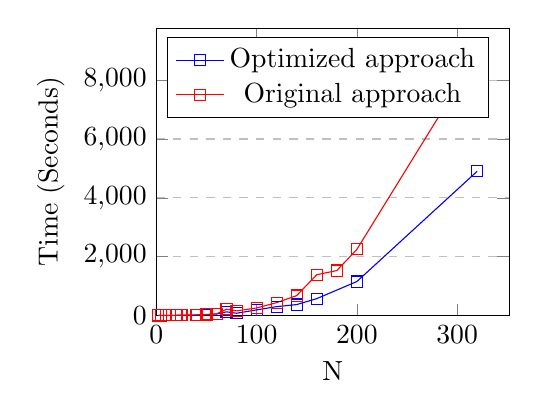
\begin{tikzpicture}
    \begin{axis}[width=0.5\textwidth,legend pos=north west,
        xlabel={N},
        ylabel={Time (Seconds)},
        xmin=0, %xmax=160,
        ymin=0, %ymax=580,
        %xtick={0,2,5,10,20,40,50,60,80,100,120,160},
        %ytick={0,20,40,60,80,100,120},
      %  legend pos=north west,
        ymajorgrids=true,
        grid style=dashed,
     %   legend style={font=\fontsize{40}{50}\selectfont}, 
    ]
    \addplot[
        color=blue,
        mark=square,
    ]
    coordinates {
    (2,0.4)(5,0.9)(10,1.8)(20,4.0)(25,7.9)(40,12.1)(50,29.1)(60,48.2)(70,122.8)(80,74.6)(100,188.4)(120,300.0)(140,369.7)(160,571.8)(200,1152.8)(320,4899.962)
    };
    \addlegendentry{Optimized approach}
    \addplot[
        color=red,
        mark=square,
    ]
    coordinates {
    (2,0.4)(5, 1.1)(10,2.1)(20,5.2)(25,8.6)(40,22.4)(50,33.8)(60,55.7)(70,210.3)(80,154.5)(100,254.1)(120,436.2)(140,675.4)(160,1385.3)(180,1525.2)(200,2245.1)(320,8876.4)
    };
   \addlegendentry{Original approach}
\end{axis}
\end{tikzpicture}}

\newcommand{\cctime}{
%Time spent to calculate the coloring semantics of N-Sequencer
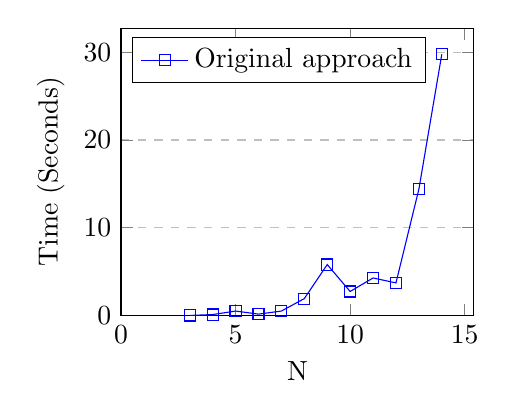
\begin{tikzpicture}
    \begin{axis}[
        width=0.5\textwidth,
        legend pos=north west,
        xlabel={N},
        ylabel={Time (Seconds)},
        xmin=0, %xmax=160,
        ymin=0, %ymax=580,
        %xtick={0,2,5,10,20,40,50,60,80,100,120,160},
        %ytick={0,20,40,60,80,100,120},
     %   legend pos=north west,
        ymajorgrids=true,
        grid style=dashed,
     %   legend style={font=\fontsize{40}{50}\selectfont},
    ]
    \addplot[
        color=blue,
        mark=square,
        ]
        coordinates {
        (3,0)(4,0.1)(5,0.5)(6,0.15)(7,0.5)(8,1.92)(9,5.8)(10,2.73)(11,4.27)(12,3.71)(13,14.39)(14,29.76)
        };
       \addlegendentry{Original approach}
    \end{axis}
\end{tikzpicture}
}

\newcommand{\catime}{
\begin{tikzpicture}
    \begin{axis}[
        width=0.5\textwidth,
        legend pos=north west,
        xlabel={N},
        ylabel={Time (Milliseconds)},
        xmin=0, %xmax=160,
        ymin=0, %ymax=580,
        %xtick={0,2,5,10,20,40,50,60,80,100,120,160},
        %ytick={0,20,40,60,80,100,120},
   %     legend pos=north west,
        ymajorgrids=true,
        grid style=dashed,
     %   legend style={font=\fontsize{40}{50}\selectfont}]
        \addplot[
            color=blue, 
            mark=square
        ]
        coordinates {(3,0)(4,0.1)(5,0.5)(6,0.15)(7,0.5)(8,24)(9,1)(10,2)(11,1    )(12,43)(13,14.39)(20,23)
        };
    \end{axis}
\end{tikzpicture}
}

\newcommand{\cacctime}{
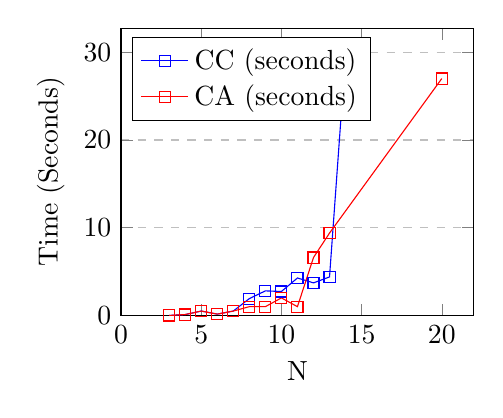
\begin{tikzpicture}
    \begin{axis}[
        width=0.5\textwidth,
        legend pos=north west,
            xlabel={N}, 
            ylabel={Time (Seconds)},
            xmin=0, %xmax=160,
            ymin=0, %ymax=580,
            %xtick={0,2,5,10,20,40,50,60,80,100,120,160},
            %ytick={0,20,40,60,80,100,120},
            legend pos=north west, 
            ymajorgrids=true, 
            grid style=dashed,
          %  legend style={font=\LARGE}
        ]
        \addplot[
            color=blue, 
            mark=square
        ]
        coordinates{(3,0)(4,0.1)(5,0.5)(6,0.15)(7,0.5)(8,1.92)(9,2.8)(10,2.73)(11,4.27)(12,3.71)(13,4.39)(14,29.76)
        };
       \addlegendentry{CC (seconds)}
       \addplot[color=red, mark=square]
        coordinates {(3,0)(4,0.1)(5,0.5)(6,0.15)(7,0.5)(8,1)(9,1)(10,2)(11,1)(12,6.6)(13,9.39)(20,27)
        };
       \addlegendentry{CA (seconds)}
    \end{axis}
\end{tikzpicture}
}
